\section{Erläuterung}

Dieser Abschnitt erläutert grundlegend die von Microsoft entwickelte Toolbox zum Thema Inklusive Design.
Dabei wird zunächst das Problem eingeschränkter Menschen mit vielen Anwendungen benannt.
Daraufhin werden Kontexte und Situationen benannt, in denen mit aufmerksamer Entwicklung Ausgrenzung vermieden werden kann.

\begin{quote}
"Eingeschränktheit entsteht an den Punkten der Interaktion zwischen Mensch und Gesellschaft.
Körperliche, kognitive und soziale Ausgrenzung ist das Ergebnis unangepasster Interaktionen." \cite{ITToolkit}
\end{quote}

Die Sicht auf körperliche Beeinträchtigungen als Fehler am Menschen ist veraltet.
An seine Stelle tritt eine neue Sicht, welche Beeinträchtigungen als kontextual begründet sieht.
Muss einem Rollstuhlfahrenden beim Einstieg in die Tram geholfen werden, so liegt dies nicht an der Person, sondern an einem fehlenden ebenerdigen Einstieg in das Transportmittel.
Ebenso verhält es sich im Gebiet der Softwareentwicklung.

Dabei wird zwischen drei Typen an Einschränkungen unterschieden:
Permanente Einschränkungen, wie beispielsweise ein amputierter Arm, Temporäre Einschränkungen, wie beispielsweise ein gebrochener Arm und Situative Einschränkungen, wie beispielsweise ein Elternteil, welches ein Baby im Arm trägt.
Oft wird Inklusion in der Software nicht umgesetzt, da ein hoher Aufwand in der Entwicklung nur einem kleinen Teil an Menschen zu Gute kommt.
Betrachtet man jedoch permanente, temporäre und situative Einschränkungen, so hilft jede inklusive Funktion mehr Menschen als im ersten Moment gedacht.

\subsection{Support Cards}

Um die Entwicklung von inklusiver Software zu unterstützen, hat Microsoft "Support Cards" entwickelt.
Diese behandeln jeweils Kontexte und Situationen, in denen Ausgrenzung auftreten kann.
Mit Hilfe der Karten können Entwickelnde prüfen, in welchem Umfang ihre Software inklusiv ist.
Diese Karten seien im Folgenden aufgelistet und kurz beschrieben.

\subsubsection{Physical Context}

Diese Karte regt die Entwickelnden an über das physische Umfeld potenzieller  Nutzenden nachzudenken.
Dabei sollte das Produkt möglichst an jedem Ort einsetzbar sein.
Es soll Zuhause am eigenen Schreibtisch, jedoch auch an anderen Orten, beispielsweise ohne Internet funktionieren.

\subsubsection{Social Context}

Ebenso soll das Produkt in jeglichen sozialen Kontexten einsetzbar sein.
Somit muss eine Einzelperson allein das Produkt bedienen können.
Gleichzeitig muss dies mit Kollegen oder Freunden und Familie funktionieren.
Ein letzter Punkt ist beispielsweise die Nutzung in einer Menschenmenge.
Hier ist die Nutzung beispielsweise durch Bewegungen und Lautstärke gestört.

\subsubsection{Temporary/Situational Limit}

Diese Karte bezieht sich auf Einschränkungen aller Art.
Dabei soll Software offen für Menschen sein, welche nicht sehen, sprechen, hören oder berühren können.
An diesem Punkt kommt ebenso die Beachtung von temporären und situativen Einschränkungen zum Tragen.
Eine Übersicht über einige Arten der Beeinträchtigung ist \autoref{fig:ways-of-disability} zu entnehmen.

\begin{figure}[htp]
    \centering
    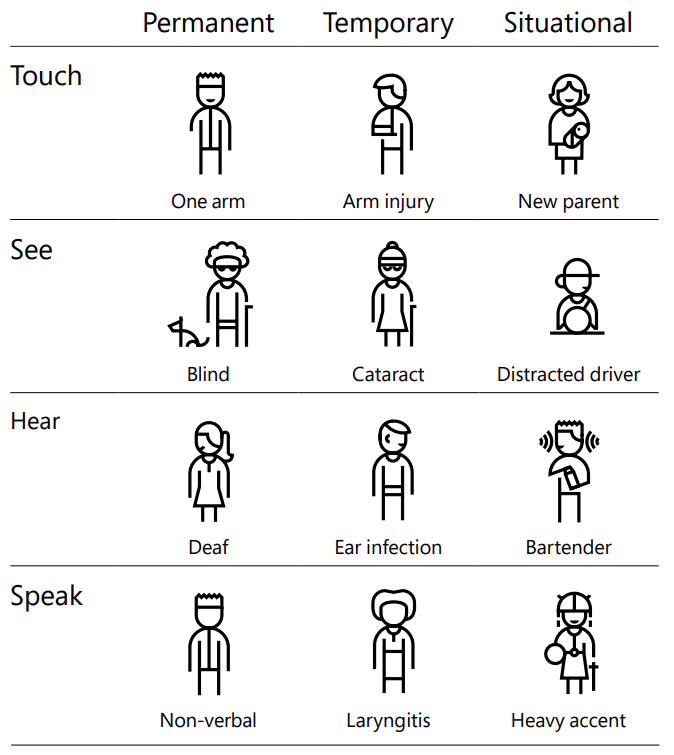
\includegraphics[width=.8\textwidth]{images/ID-disabilities.png}
    \caption{Arten von Eingeschränktheit \cite{ITToolkit}}
    \label{fig:ways-of-disability}
\end{figure}

\subsubsection{Role of Technology}

Wenn eine Software entwickelt werden soll, so soll diese eine Rolle einnehmen.
Beispielrollen sind Sammeln, Zusammenfassen, Übersetzen, Transportieren und Hören.
Im Zuge der Entwicklung sollen die Entwickler darauf achten, dass ihre Software die anfangs geforderte Rolle(n) einnimmt und nicht darüber hinaus arbeitet.
Dies steht in direkter Verbindung zu der in \autoref{sec:definition} erwähnten Aufgabenangemessenheit.

\subsubsection{Conditions}

Letztlich soll Software bei allen Bedingungen nutzbar sein.
Hierbei geht es beispielsweise um Wetter, Temperatur, aber auch Tageszeit.
Viele Nutzenden finden bei nächtlicher Arbeit beispielsweise das Angebot eines Blaufilters auf der Software für angemessen.

